		%%%%%%%%%%%%%%%%%%%%%%%%%%%%%%%%%%%%%%%%%
		% Beamer Presentation
		% LaTeX Template
		% Version 1.0 (10/11/12)
		%
		% This template has been downloaded from:
		% http://www.LaTeXTemplates.com
		%
		% License:
		% CC BY-NC-SA 3.0 (http://creativecommons.org/licenses/by-nc-sa/3.0/)
		%
		%%%%%%%%%%%%%%%%%%%%%%%%%%%%%%%%%%%%%%%%%
		
		%----------------------------------------------------------------------------------------
		%	PACKAGES AND THEMES
		%----------------------------------------------------------------------------------------
		
		\documentclass[professionalfont,fleqn]{beamer}
		% \documentclass[9pt, handout]{beamer} ## Esto es para armar una versión compacta para circular
		\setbeamercovered{transparent}
		\setlength{\mathindent}{0pt}
		
		\mode<presentation> {
		
		% The Beamer class comes with a number of default slide themes
		% which change the colors and layouts of slides. Below this is a list
		% of all the themes, uncomment each in turn to see what they look like.
		
		\usetheme{Luebeck}
		%\usetheme{Madrid}
		%%\usetheme{Malmoe}
		%\usetheme{Marburg}
		%%\usetheme{Montpellier}
		%\usetheme{PaloAlto}
		%%\usetheme{Pittsburgh}
		%\usetheme{Rochester}
		%\usetheme{Singapore}
		%\usetheme{Szeged}
		%\usetheme{Warsaw}
		
		% As well as themes, the Beamer class has a number of color themes
		% for any slide theme. Uncomment each of these in turn to see how it
		% changes the colors of your current slide theme.
		
		%\usecolortheme{albatross}
		%%\usecolortheme{beaver}
		%\usecolortheme{beetle}
		%\usecolortheme{crane}
		%\usecolortheme{dolphin}
		%%\usecolortheme{dove}
		%\usecolortheme{fly}
		%\usecolortheme{lily}
		%\usecolortheme{orchid}
		%\usecolortheme{rose}
		%\usecolortheme{seagull}
		\usecolortheme{seahorse}
		%\usecolortheme{whale}
		%\usecolortheme{wolverine}
		
		%\setbeamertemplate{footline} % To remove the footer line in all slides uncomment this line
		%\setbeamertemplate{footline}[page number] % To replace the footer line in all slides with a simple slide count uncomment this line
		
		%\setbeamertemplate{navigation symbols}{} % To remove the navigation symbols from the bottom of all slides uncomment this line
		}
		\usepackage{amssymb}
		\usepackage{amsmath}
		
		\usepackage{graphicx}
		\graphicspath{ {Graficos/} }
		\usepackage{subfigure}
		\usepackage{booktabs} % Allows the use of \toprule, \midrule and \bottomrule in tables
		\usepackage[utf8]{inputenc}
		\usepackage[spanish]{babel}
		
		
		\newcommand*{\boxedcolor}{red}
		\makeatletter
		\renewcommand{\boxed}[1]{\textcolor{\boxedcolor}{%
				\fbox{\normalcolor\m@th$\displaystyle#1$}}}
		\makeatother
		
		%----------------------------------------------------------------------------------------
		%	TITLE PAGE
		%----------------------------------------------------------------------------------------
		
		\title[Grafo de Comercio internacional]{Descripción del comercio internacional utilizando un modelo de redes complejas con igraph} % The short title appears at the bottom of every slide, the full title is only on the title page
		
		\author{Diego Kozlowski} % Your name
		\institute[Universidad de Buenos Aires] % Your institution as it will appear on the bottom of every slide, may be shorthand to save space
		{
		Universidad de Buenos Aires\\ % Your institution for the title page
		\medskip
		mail: \textit{diegokoz92@gmail.com} % Your email address
		\\
		twitter: \textit{@Diego\_Koz}
		}
		\date{5 de septiembre 2018} % Date, can be changed to a custom date
		
		\begin{document}
		
		\begin{frame}
		\titlepage % Print the title page as the first slide
		\end{frame}
		
		
		\begin{frame}
		\frametitle{Introducción}
		\begin{itemize}
			\item El comercio internacional como un grafo
			\item Decisiones metodológicas asociadas a esta representación
			\item Expresiones de la Nueva División Internacional del Trabajo
		\end{itemize}
		
		\end{frame}
		
		%\begin{frame}
		%\frametitle{Overview} % Table of contents slide, comment this block out to remove it
		%\tableofcontents % Throughout your presentation, if you choose to use \section{} and \subsection{} commands, these will automatically be printed on this slide as an overview of your presentation
		%\end{frame}
		
		%----------------------------------------------------------------------------------------
		%	PRESENTATION SLIDES
		%----------------------------------------------------------------------------------------
		
		%------------------------------------------------
		\section{Metodología} % Sections can be created in order to organize your presentation into discrete blocks, all sections and subsections are automatically printed in the table of contents as an overview of the talk
		%------------------------------------------------
	
	
		
		\begin{frame}
		\frametitle{Data}
		
		Datos de comercio bilateral agregado entre países, por año		
		\vspace*{10pt}
		
		\textit{Fuentes:}  
		\begin{itemize}
			\item {Gleditsch 1950-2000}\footnote{\url{http://privatewww.essex.ac.uk/~ksg/exptradegdp.html}}
			\item {Comtrade. 1997-2011}\footnote{\url{https://comtrade.un.org/}}
		\end{itemize}
		
		\end{frame}
		
		%\subsection{Construction of the network} % A subsection can be created just before a set of slides with a common theme to further break down your presentation into chunks
		\begin{frame}
		\frametitle{Comercio Bilateral}
		
		\begin{columns}[t]
			\column{.5\textwidth}
			
				\begin{equation*}
				a_{ij} = 
				\begin{cases} 
				1 & si \ \frac{x_{ij}}{x_{i\cdot}}\geq u \\
				0 & sino 
				\end{cases}
				$$
				\end{equation*}
				$x_{ij}$: Comercio total entre los países i-j \par
				$x_{i\cdot}$: Comercio total del país i
			
			\column{.5\textwidth}
			
			\begin{itemize}
				\item Dos países están conectados si existe \textit{suficiente} comercio entre ellos.
				\item Puede ser tanto expo como impo.
				\item El grafo es dirigido, por lo que $a_{ij} \neq a_{ji}$.
			\end{itemize}
			
		\end{columns}
		
		\end{frame}
		
				
		
\begin{frame}
\frametitle{Productores \& Consumidores}	
	\begin{columns}
		\column{.5\textwidth}
			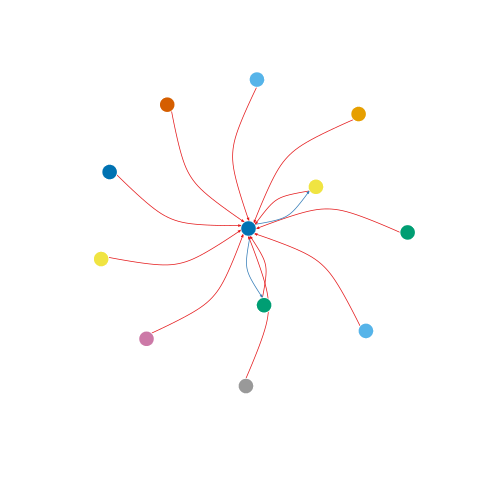
\includegraphics[width=\linewidth]{toy_graph1}
		
		\column{.65\textwidth}
		\begin{itemize}
			\item Desde el punto de vista de un país, no puede haber muchos países relevantes, $\therefore$ no hay muchas \textbf{aristas de salida}
			\item Pero puede ser relevante desde el punto de vista de muchos otros países.
			$\therefore$ puede recibir muchas \textbf{aristas de entrada}
			\item Con datos de \textbf{expo}, un nodo central es \textbf{importante como consumidor}
			\item Con datos de \textbf{impo}, un nodo central es \textbf{importante como productor}
		\end{itemize}	
	\end{columns}	
\end{frame}
		
\begin{frame}
\frametitle{Productores \& Consumidores}	
\begin{columns}
	\column{.5\textwidth}
	\hspace*{-0.2\linewidth}
	\includegraphics<1>[width=1.5\linewidth]{grafo_2016_1_pcnt}
	%\hspace*{-0.2\linewidth}
	\includegraphics<2>[width=1.5\linewidth]{grafo_2016_20_pcnt}
	
	\column{.5\textwidth}
	\begin{itemize}
		\item<1-> Con datos reales.
		\item<1> Con un punto de corte 1\% , este fenómeno no es apreciable. 
		\item<2-> Con 20\%, Podemos ver algunos nodos importantes con muchas \textbf{aristas de entrada}
	\end{itemize}	
\end{columns}	
\end{frame}
	%------------------------------------------------
		
		\section{Resultados}
	
		\begin{frame}
	\frametitle{Representación gráfica}
	
	
		\begin{onlyenv}<1>
			%Threshold: 1\%
			\begin{center}
			\includegraphics<1>[width=.75\textwidth,height=.75\textwidth]{grafo_Circ_2011_1_pcnt}
			\end{center}
		\end{onlyenv}
	
				
	\begin{columns}[t]
		\column{.5\textwidth}
		\centering
		\includegraphics<2->[width=.7\linewidth,height=.7\linewidth]{grafo_Circ_2011_1_pcnt}\\
		%\only<2->{\texttt{1\%}}
		\includegraphics<2->[width=.7\linewidth,height=.7\linewidth]{grafoCirc_2011_5_pcnt}
		%\only<2->{\texttt{5\%}}
		\column{.5\textwidth}
		\centering
		\includegraphics<3->[width=.7\linewidth,height=.7\linewidth]{grafoCirc_2011_10_pcnt}\\
		%\only<3->{\texttt{10\%}}
		\includegraphics<4->[width=.7\linewidth,height=.7\linewidth]{grafoCirc_2011_15_pcnt}
		%\only<4->{\texttt{15\%}}
	\end{columns}
	
	\end{frame}
	
		
	\begin{frame}
		\frametitle{Correlación de Expo e Impo I}
		
		
		\textbf{Centralidad de grado} en el grafo de impo respecto del de expos
		\begin{columns}[c] % The "c" option specifies centered vertical alignment while the "t" option is used for top vertical alignment
	%			
		\column{.6\textwidth} % Right column and width
		\begin{flushleft}
			\begin{figure}
				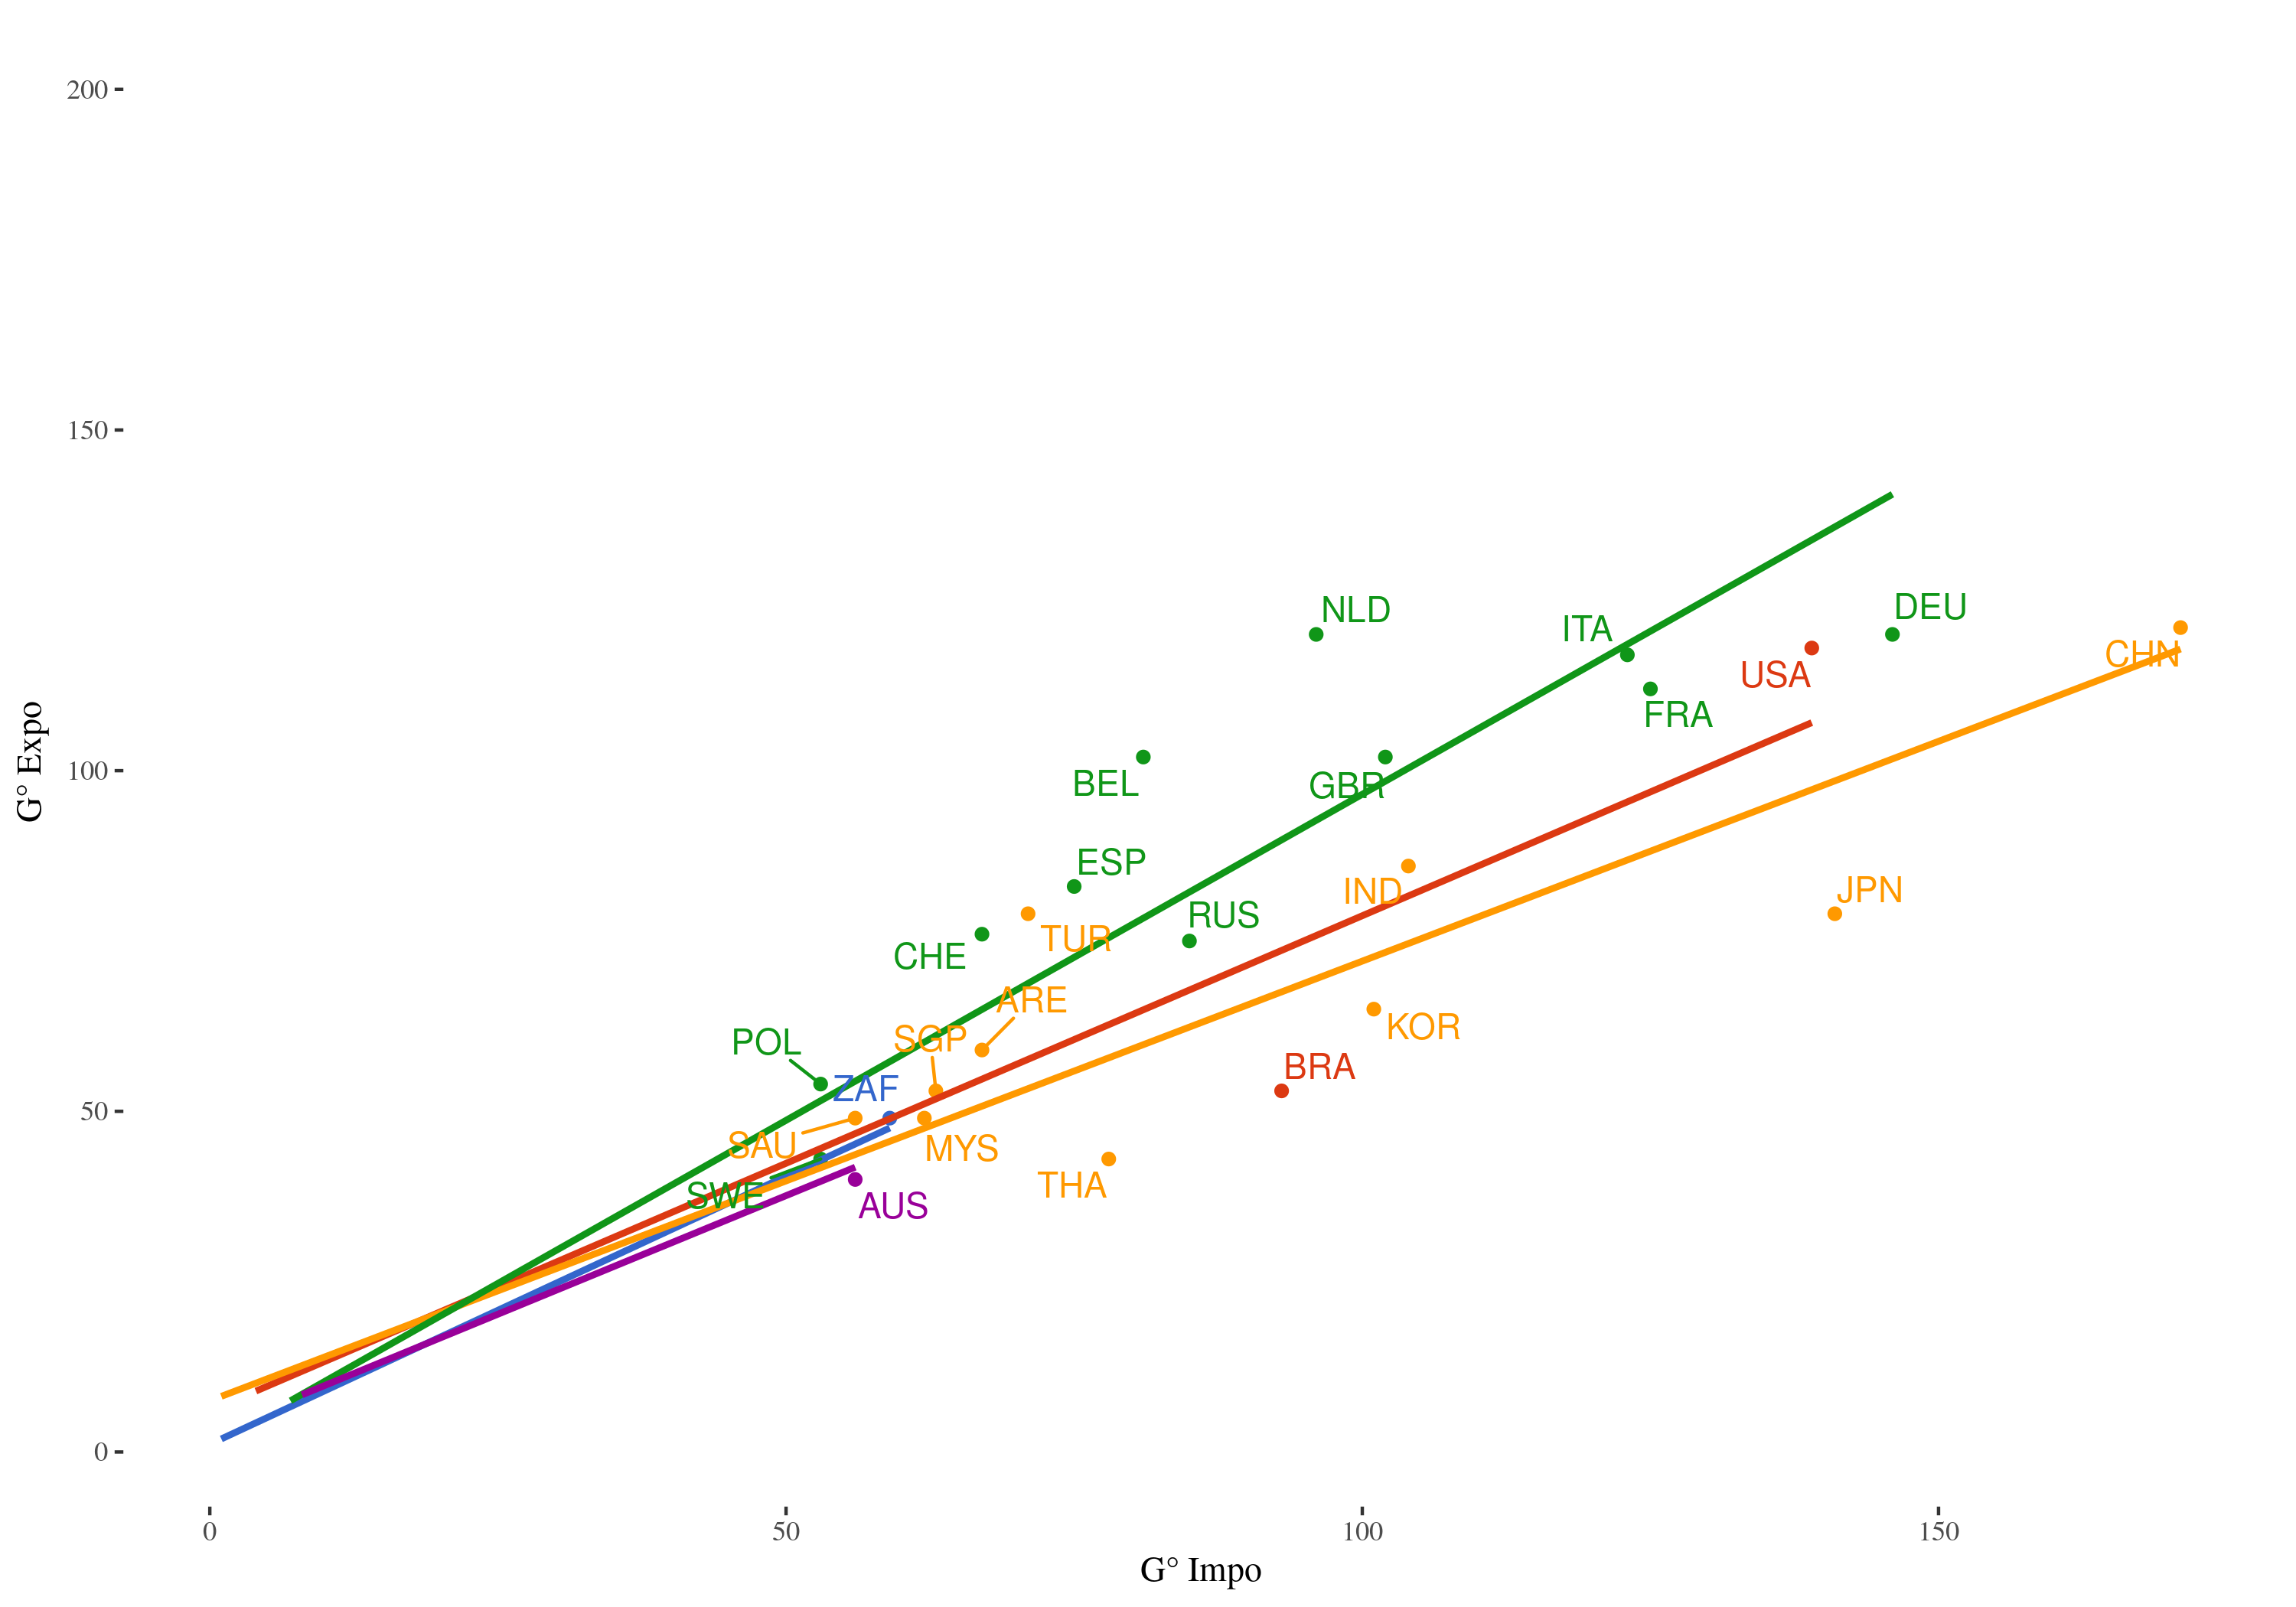
\includegraphics[width=\linewidth]{corr_grados_2011_1_pcnt}
			\end{figure}
		\end{flushleft}
		
		
		\column{.45\textwidth} % Left column and width
		\begin{itemize}
			\item 1\% Threshold: Red de baja dependencia.
			\item Europa es más importante como consumidora.
			\item Asia es más centra como productora.
		\end{itemize}
		\end{columns}
	\end{frame}
	%%%%%	
			\begin{frame}
		\frametitle{Correlación de Expo e Impo II}
		\begin{columns}[c] % The "c" option specifies centered vertical alignment while the "t" option is used for top vertical alignment
			
		
		\column{.65\textwidth} % Right column and width
		\begin{flushleft}
			\begin{figure}
				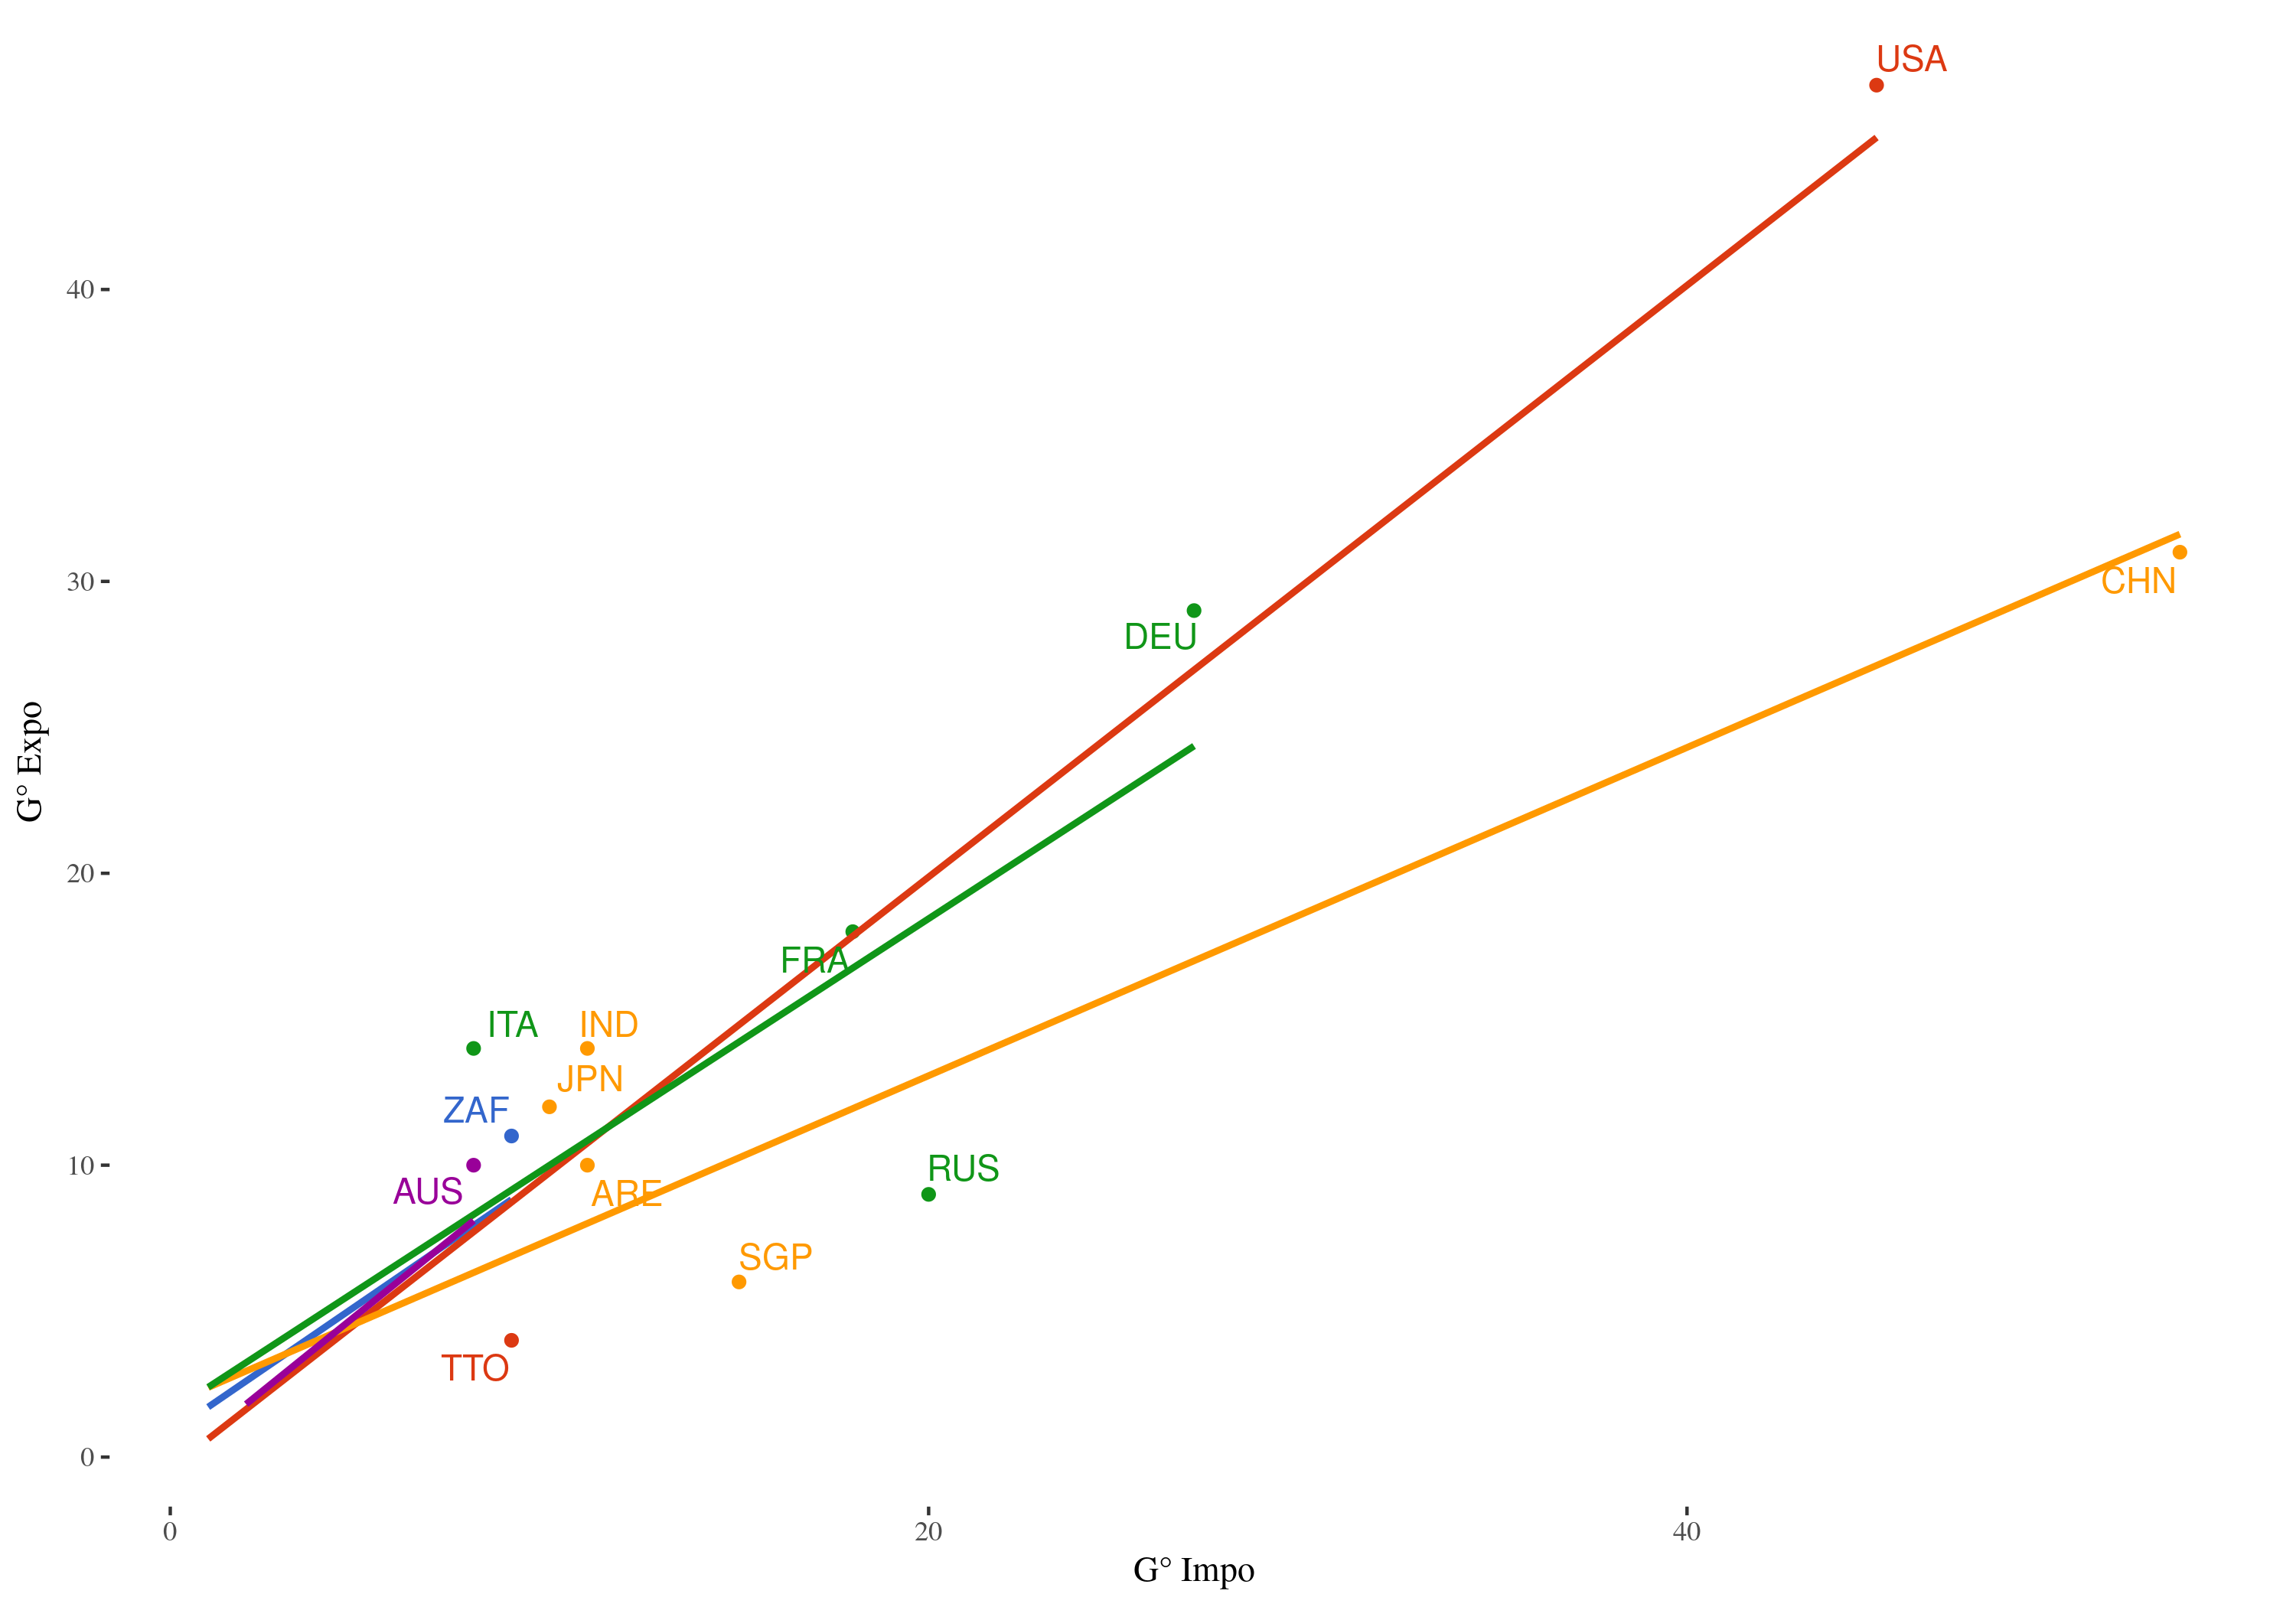
\includegraphics[width=\linewidth]{corr_grados_2011_10_pcnt}
			\end{figure}
		\end{flushleft}
		
		
		\column{.45\textwidth} % Left column and width
		\begin{itemize}
			\item 10\% Threshold.
			\item EEUU y Alemania se comienzan a separar de los demás nodos, con mayor relevancia como consumidores.
			\item China también resalta, como productora.
		\end{itemize}
		\end{columns}
	\end{frame}
		\begin{frame}
		
	\frametitle{Correlación de Expo e Impo III}
		\begin{columns}[c] % The "c" option specifies centered vertical alignment while the "t" option is used for top vertical alignment
		
	
	
	\column{.65\textwidth} % Right column and width
	\begin{flushleft}
		\begin{figure}
			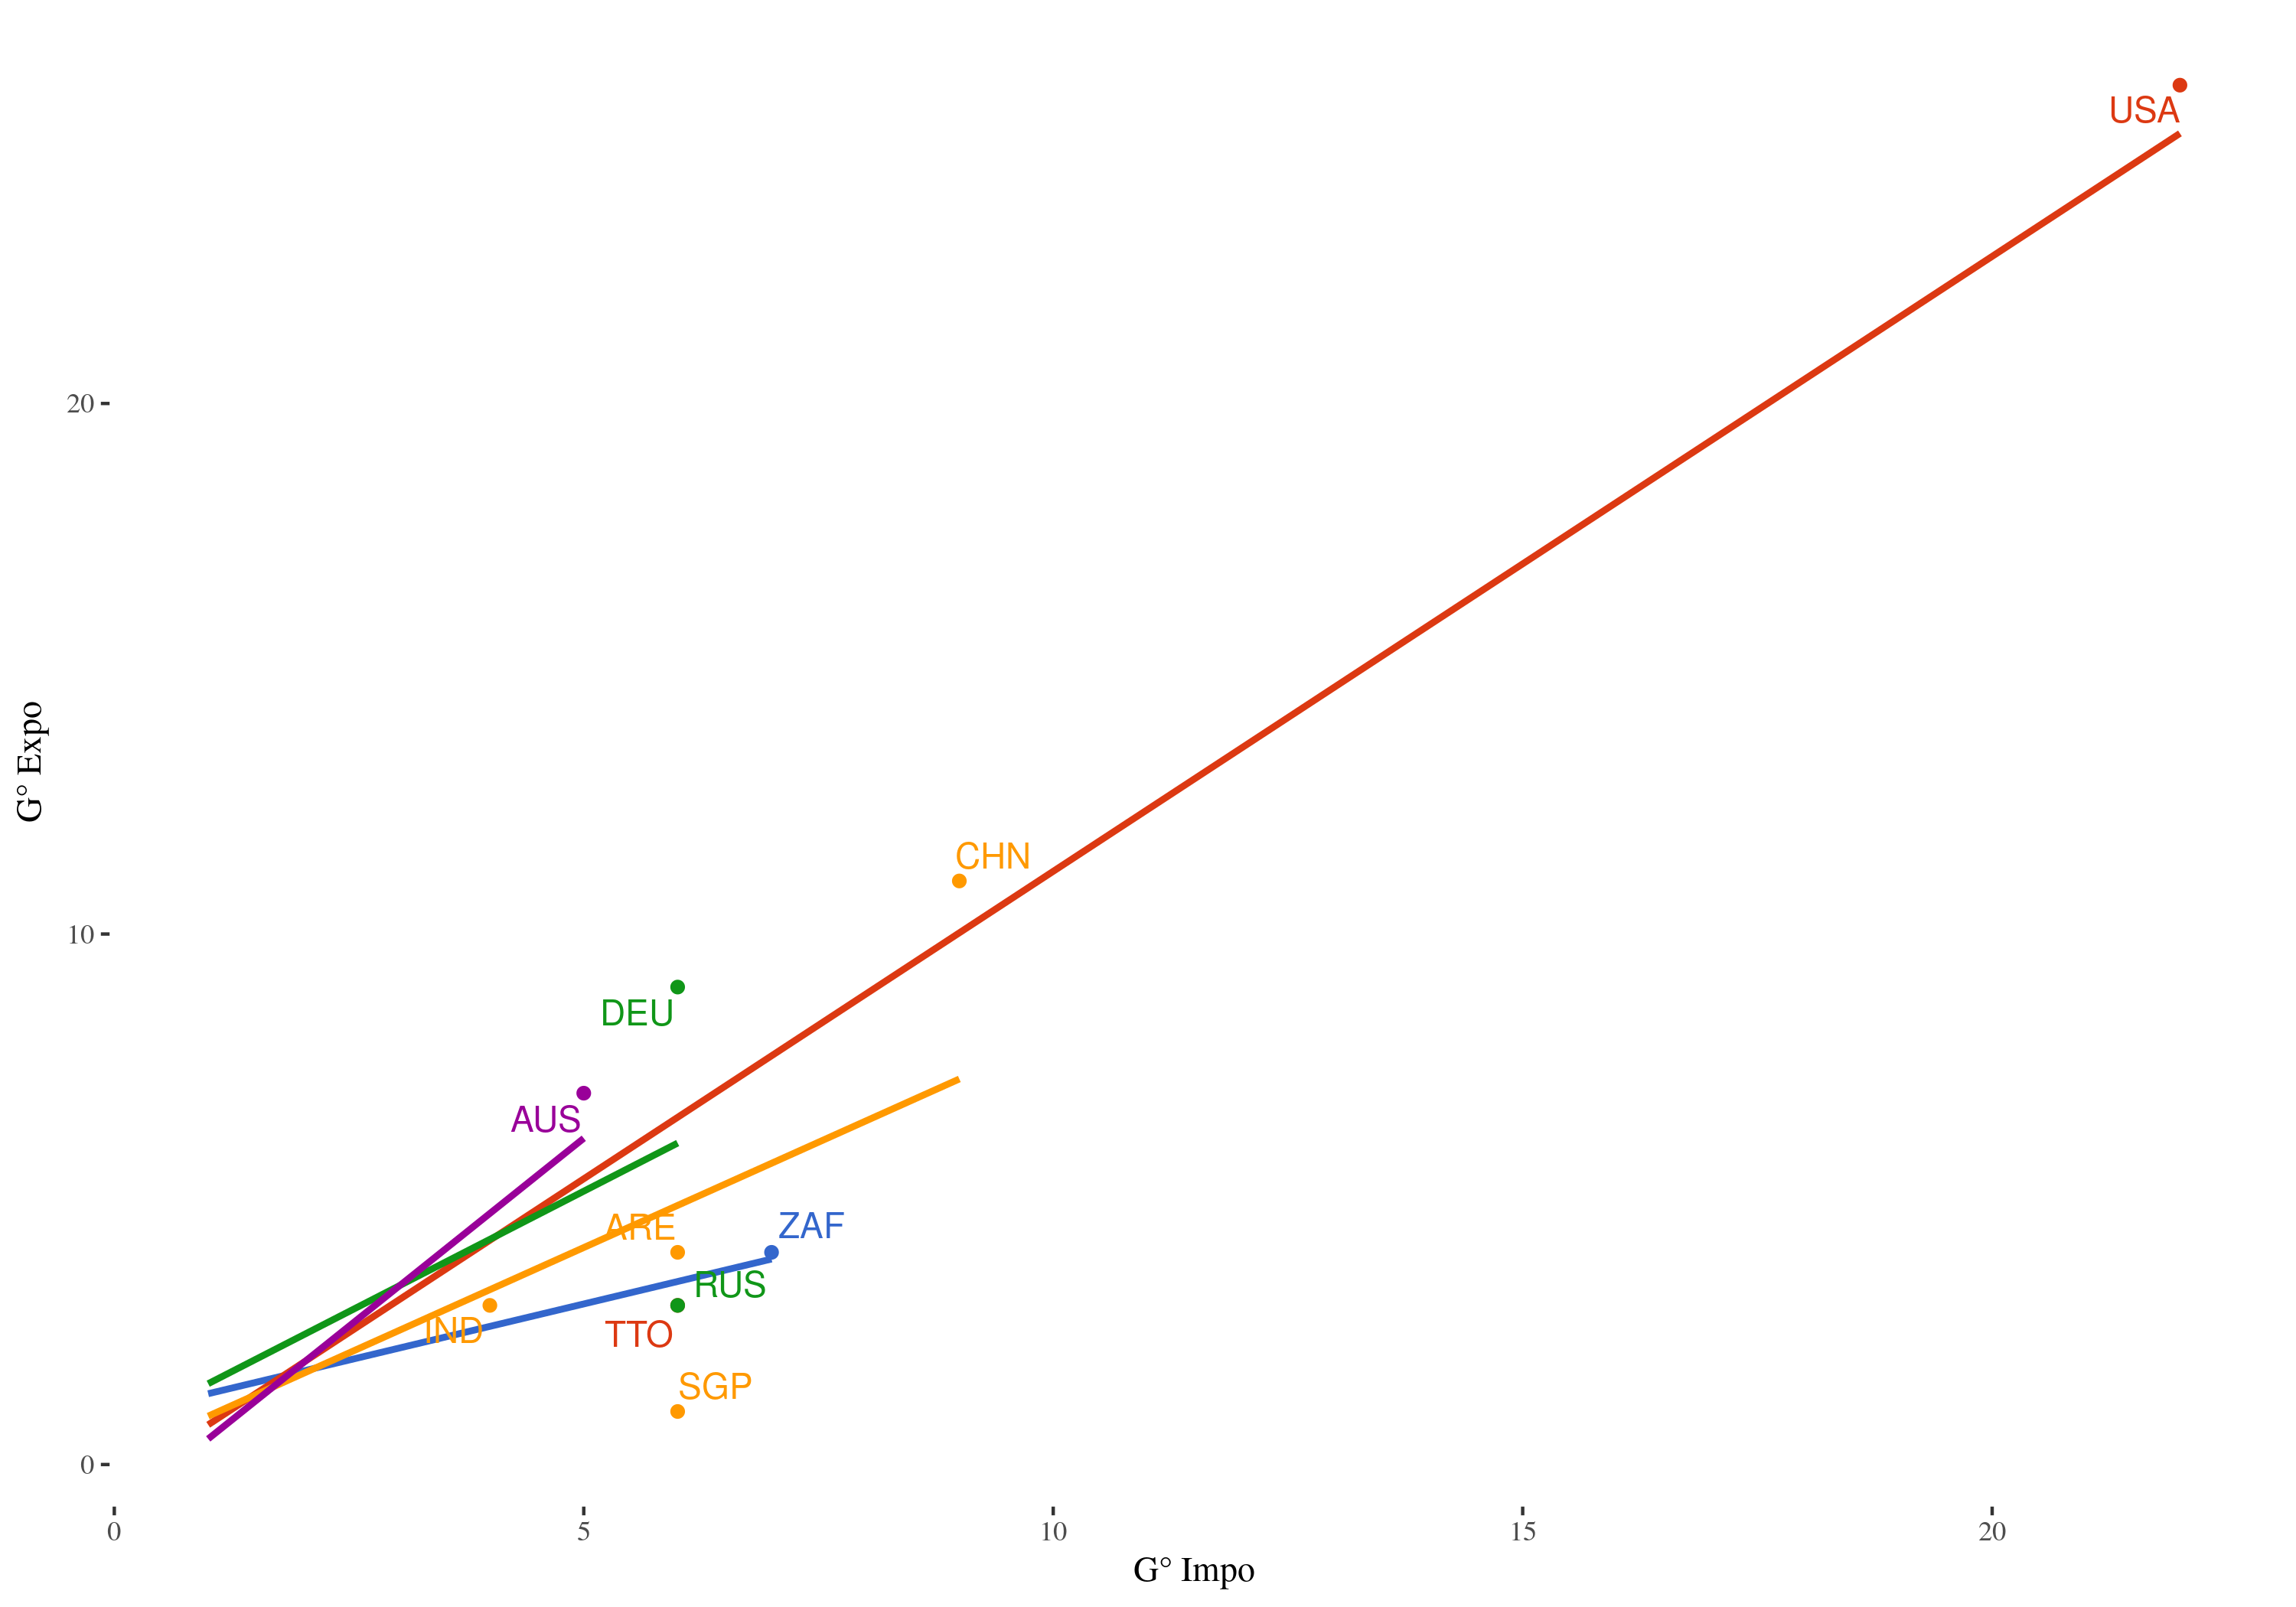
\includegraphics[width=\linewidth]{corr_grados_2011_20_pcnt}
		\end{figure}
	\end{flushleft}
	
	
	\column{.45\textwidth} % Left column and width
	\begin{itemize}
		\item 20\% Threshold: Red de alta dependencia.
		\item Al considerar este tipo de relaciones, EEUU tiene mucha mayor centralidad.
		\item Sudáfrica aparece como un país importante.
	\end{itemize}
		\end{columns}
	\end{frame}
	
	%------------------------------------------------
		\begin{frame}
		\frametitle{China-EEUU 1950-2000 \& 1997-2011}
		
	
		
		\begin{columns}[c] % The "c" option specifies centered vertical alignment while the "t" option is used for top vertical alignment
			
			\column{.45\textwidth} % Right column and width
				\begin{figure}
					\includegraphics<1->[scale=0.25]{1950_2000_impo_densidad_USA_CHN_grado}
				\end{figure}
			
			
			\column{.5\textwidth} % Left column and width
				\small{Podemos ver la evolución en el tiempo de la \textbf{distribución de la centralidad de grado} y el lugar de China y EEUU en el kernel.} \par
			Grado.Threshold 1\%. Impo
			\begin{flushleft}
				\begin{figure}
					\includegraphics<2->[scale=0.35]{impo_densidad_USAvsCHN_grado_x_yr}
				\end{figure}
			\end{flushleft}
			
		\end{columns}
		\end{frame}
		
		\begin{frame}
		\frametitle{Nueva División Internacional del Trabajo -I}
		\framesubtitle{Medidas Globales}
		\begin{columns}[t] % The "c" option specifies centered vertical alignment while the "t" option is used for top vertical alignment
			
			
				\column{.45\textwidth} % Right column and width
			\begin{figure}
				\vspace*{-1cm}
				\includegraphics<1->[scale=0.37]{1950_2000_coef_clustering_x_yr}
				\only<1->{Coeficiente de Clustering}
				\only<1->{ \par \small{La red reduce su regionalismo}}
			\end{figure}
			
			
			\column{.45\textwidth} % Left column and width
			\begin{flushleft}
				\begin{figure}
					\vspace*{-1cm}
					\includegraphics<2->[scale=0.4]{1950_2000_correlacion_x_yr}
					\only<2->{Coeficiente de Correlación}
					\only<2->{ \par \small{Crece el comercio entre países centrales y periféricos}}
				\end{figure}
			\end{flushleft}
		\end{columns}
		\end{frame}
		
		\begin{frame}
		\frametitle{Nueva División Internacional del Trabajo -II}
		\framesubtitle{Evolución de países}
		\begin{columns}[c] % The "c" option specifies centered vertical alignment while the "t" option is used for top vertical alignment
			
			
			\column{.35\textwidth} % Right column and width
			\begin{flushleft}
			\begin{figure}
				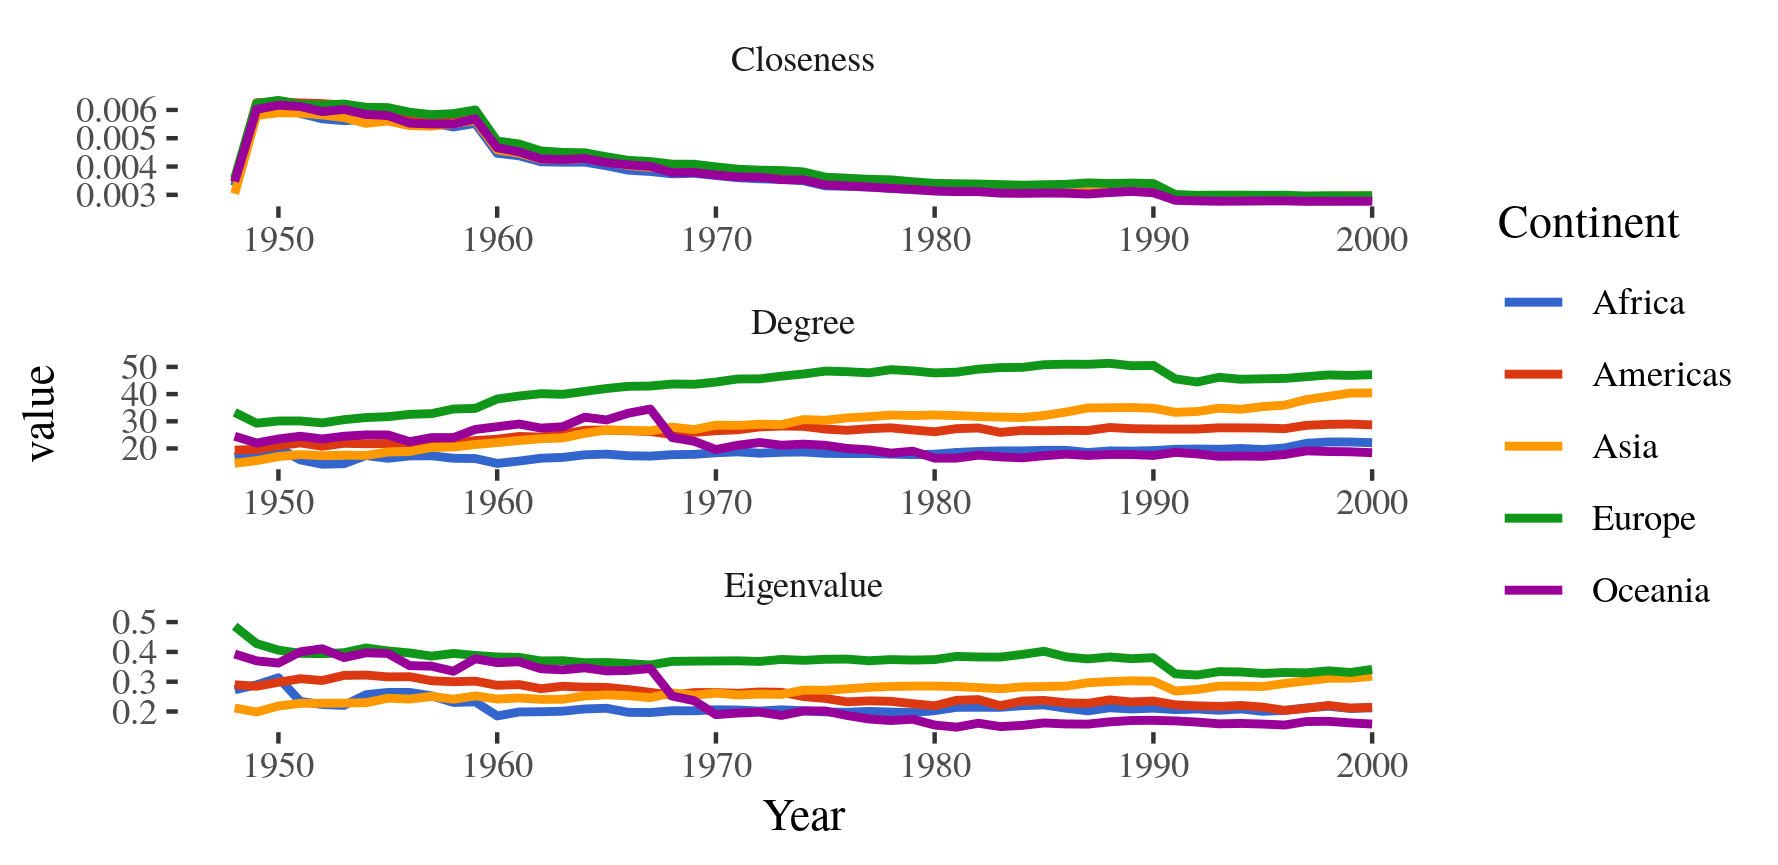
\includegraphics[width=2\linewidth]{1950_2000_continent_all_presentation}
			\end{figure}
			\end{flushleft}
			
			\column{.25\textwidth} % Left column and width\\
			
			
			\column{.45\textwidth} % Left column and width
			\begin{itemize}
				\item<1-> La cercanía promedio es una medida robusta.
				\item<2-> Asia pasa del último lugar al segundo en la centralidad de Autovalor y de Grado.
				\item<3-> Oceanía va del segundo lugar al último en esas medidas.  
			\end{itemize}
		
		\end{columns}
		\end{frame}
		
		
		\begin{frame}
		\frametitle{Nueva División Internacional del Trabajo -III}
		\framesubtitle{El rol de Asia}
		\begin{columns}[c] % The "c" option specifies centered vertical alignment while the "t" option is used for top vertical alignment
			
			
			\column{.4\textwidth} % Right column and width
			\begin{flushleft}
				\begin{figure}
					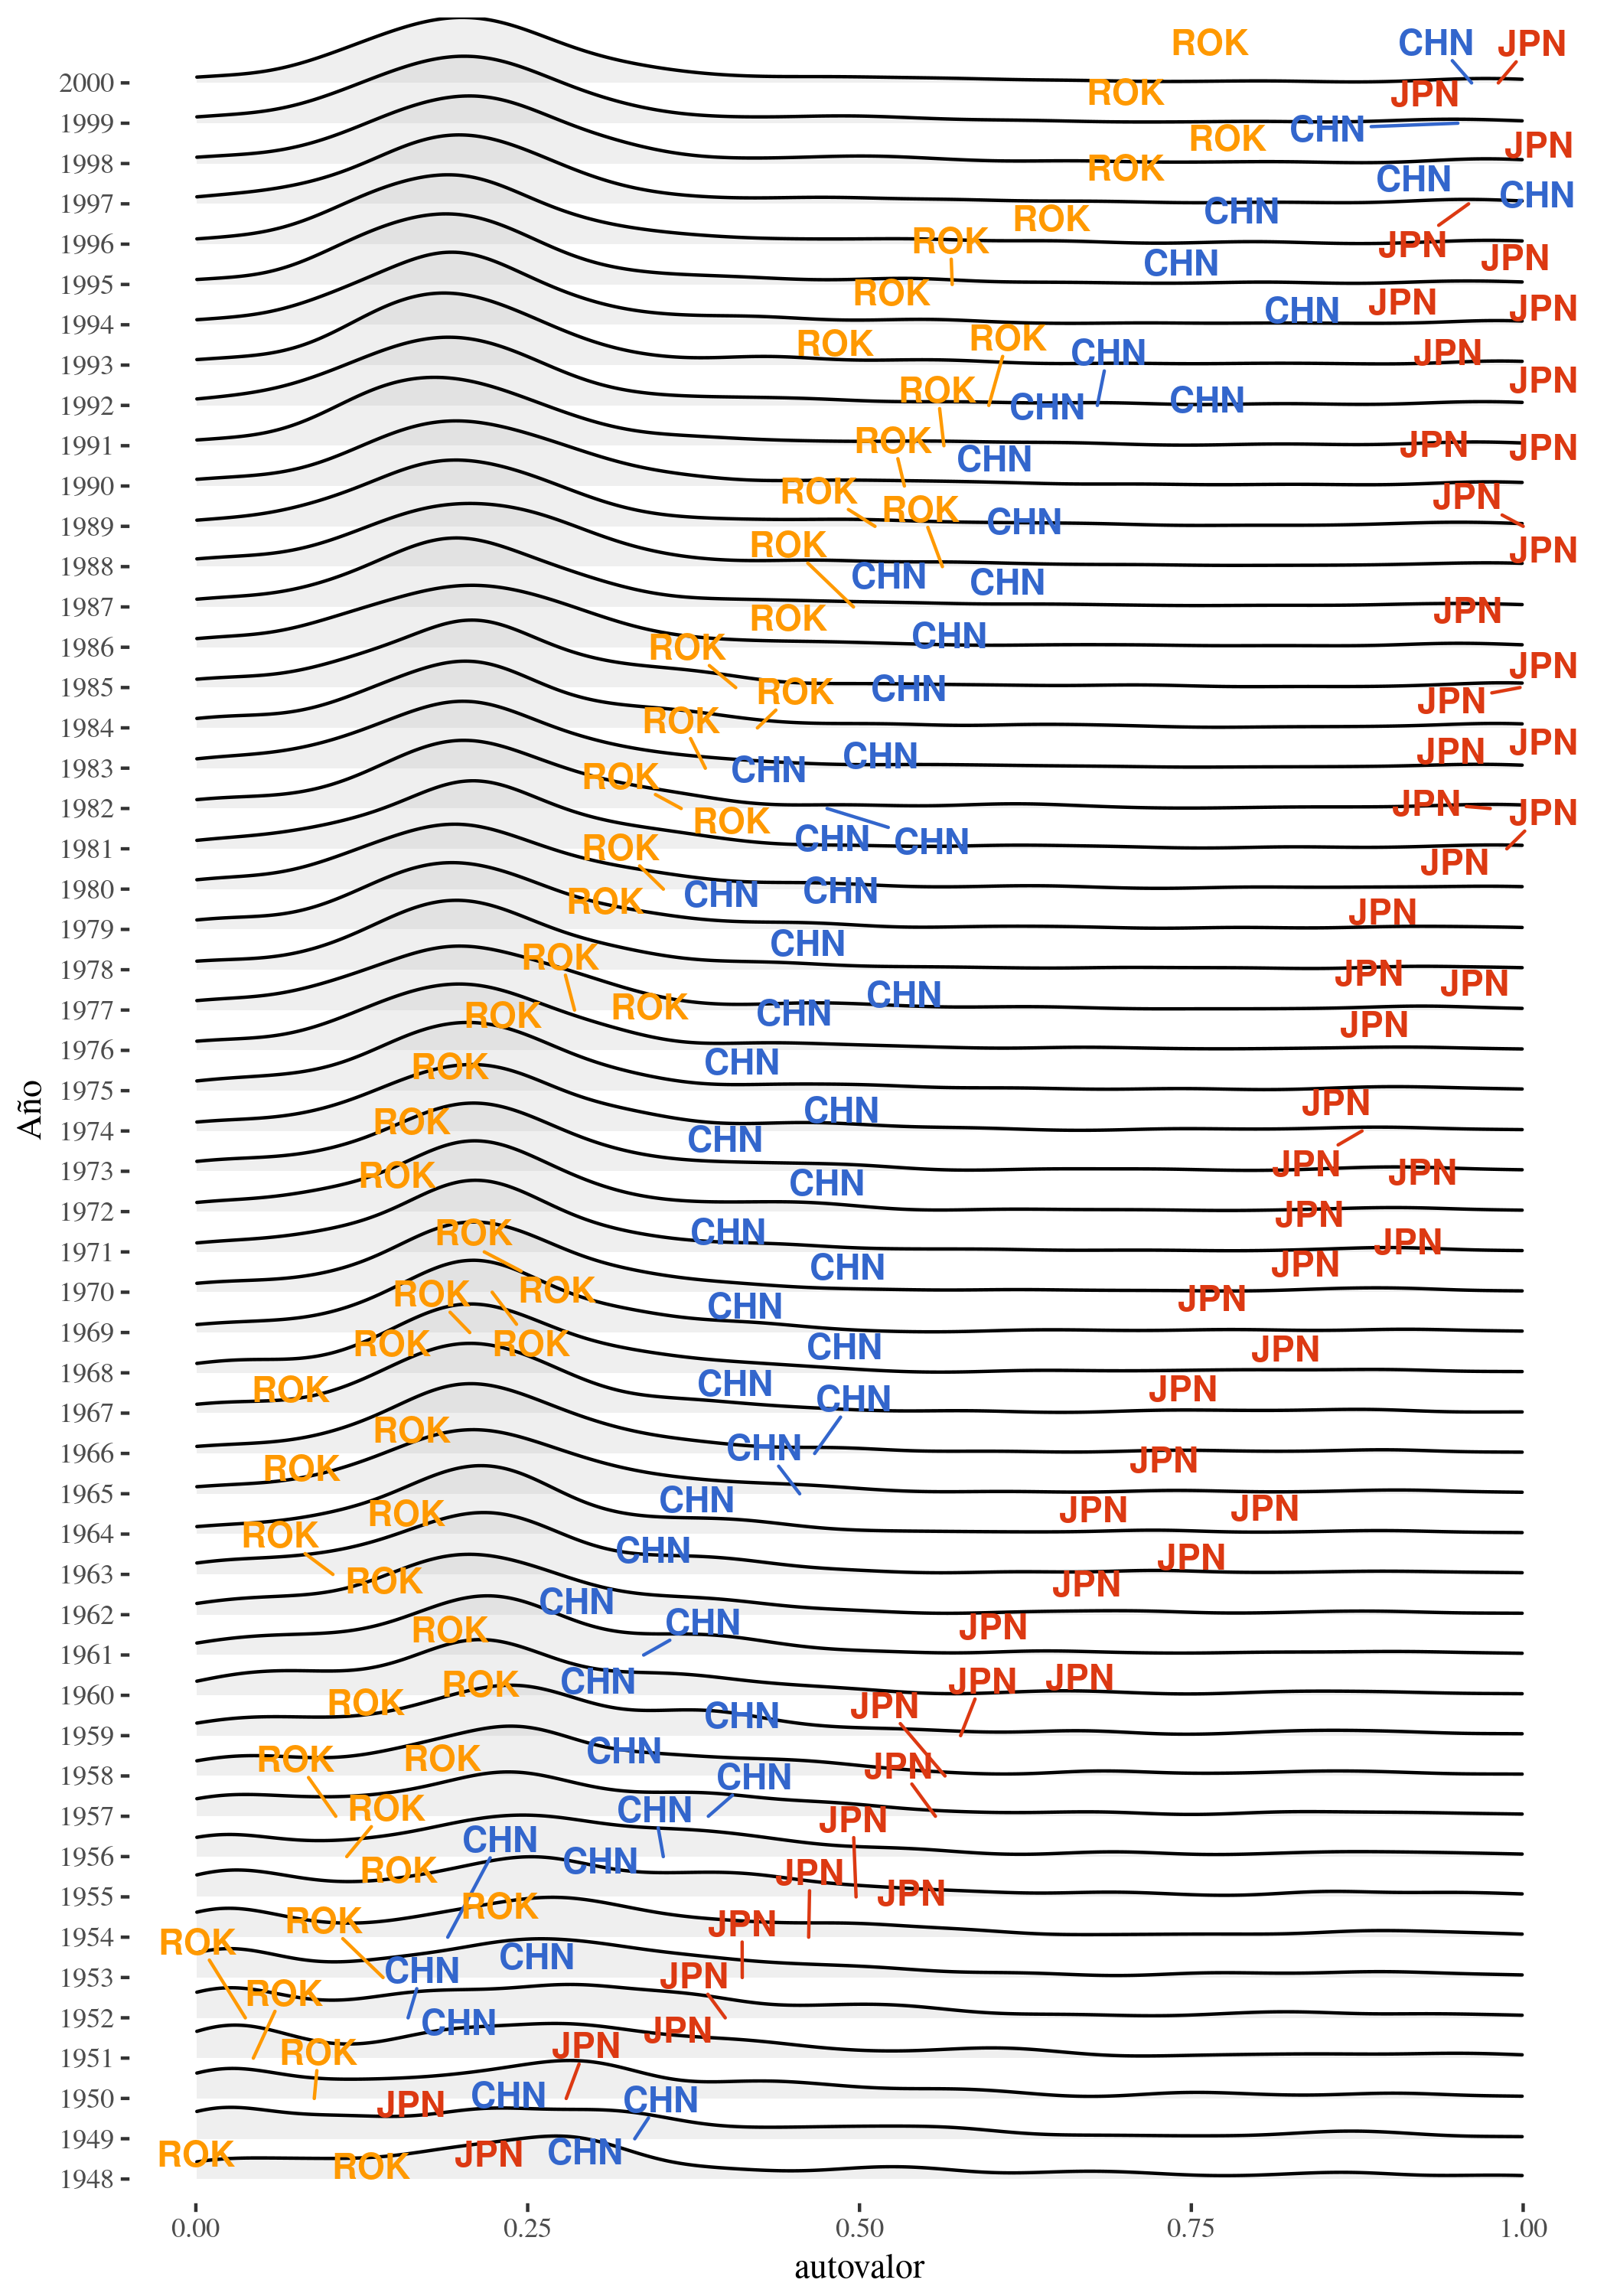
\includegraphics[width=\linewidth]{1950_2000_impo_densidad_CHN_JPN_ROK_atvlr}
					\only<1->{\small{Autovalor}}
				\end{figure}
			\end{flushleft}
			
			
			\column{.45\textwidth} % Left column and width
			\begin{itemize}
				\item<1-> Japón tiene el mismo camino al centro, varios años antes.
				\item<2-> Corea del sur también escala posiciones en el grafo, aunque empezando de más atrás.
			\end{itemize}
			
		\end{columns}
		\end{frame}
		
		\begin{frame}
		\frametitle{Nueva División Internacional del Trabajo -IV}
		\framesubtitle{América Latina}
		\begin{columns}[c] % The "c" option specifies centered vertical alignment while the "t" option is used for top vertical alignment
			
			
			\column{.45\textwidth} % Right column and width
			\begin{flushleft}
				\begin{figure}
					\includegraphics<1->[width=.9\linewidth]{1950_2000_impo_densidad_ARG_BRA_MEX_grado}
					\only<1->{\small{Grado}}
				\end{figure}
			\end{flushleft}
	
			\column{.45\textwidth} % Left column and width
	\begin{itemize}
		\item<1-> Desde los 80' Brasil aumenta la cantidad de vínculos comerciales.
		\item<2-> Argentina y México mantienen su importancia relativa durante el período.
	\end{itemize}
	
		
	\end{columns}
	\end{frame}
	
	\begin{frame}
	\frametitle{Nueva División Internacional del Trabajo -IV}
	\framesubtitle{América Latina}
	\begin{columns}[c] % The "c" option specifies centered vertical 		
			
			\column{.45\textwidth} % Left column and width
			\begin{flushleft}
			\begin{figure}
				\includegraphics<1->[width=.9\linewidth]{1950_2000_impo_densidad_ARG_BRA_MEX_atvlrpnd}
				\small{Weighted Eigenvalue}
			\end{figure}
		\end{flushleft}
			
			\column{.45\textwidth} % Left column and width
	\begin{itemize}
		\item<1-> Si se mira el autovalor ponderado por el flujo comercial, que considera la importancia de los vecinos, México crece fuerte a partir de los 90'
		\item<2-> Esto puede deberse a su relación con EEUU, conocido como \textit{Maquila Mexicana}
	\end{itemize}
	
		\end{columns}
		\end{frame}
		
		\begin{frame}
		\frametitle{Conclusiones}
		\begin{itemize}
			\item El análisis de redes tiene un gran potencial para describir el comercio mundial
			\item EEUU y Europa tienen un rol más importante como consumidores que como productores
			\item También encontramos que Asia, y China en particular, en los últimos 60 años han tenido un rol creciente en el grafo.
		\end{itemize}
		\end{frame}
	
		
		\begin{frame}
		\Huge{\centerline{Fin}}
		\vspace{1in}
		\large{\url{github.com/DiegoKoz/grafo_comercio_agregado}}
		\end{frame}
		
		%----------------------------------------------------------------------------------------
		
		\end{document}